By this point in the analysis all the selections have been finalised and discussed.
Furthermore, clear definitions for tag-$B$ mesons that properly kinematically constrain \BtoXsgamma are presented, such that \EB is evaluated accurately.
However, as can be seen \Cref{fig:spectrum_after_optimisation}, even though continuum and $\BB$ backgrounds is suppressed heavily compared to the \EB distributions that was begun with (\Cref{fig:spectrum_after_reco}),
there is still a significantly larger number of background processes than \BtoXsgamma signal events.
Many of these, particularly continuum background, originate from incorrect tag-$B$ mesons (see \Cref{fig:good_tag_definitions}) and can therefore be estimated in data using an \Mbc fitting procedure.
In this section, a thorough overview of the \Mbc fit will be presented which will extract the counts of good-$B$ tags in different \EB intervals.

\subsection{Components in the dataset}\label{sec:fitting_components}

There are three types of events in \epem collision dataset following all the selections described so far:
\begin{itemize}
    \item Generic-\BB (including \BtoXsgamma) that are tagged with a good tag-$B$;
    \item Generic-\BB (including \BtoXsgamma) that are tagged with a misreconstructed tag-$B$;
    \item Photons candidates originating in \epem\ra\qqbar.
\end{itemize}
These three components are referred to as `peaking', `combinatorial \BB' and `continuum' throughout this \Cref{sec:fitting_mbc}.
These components, extracted from generic \MC, are visualised in \Cref{fig:tag_component_fits}.

\begin{figure}[htbp!]
    \centering
    \subcaptionbox{\label{fig:good_tags_fit}}{
        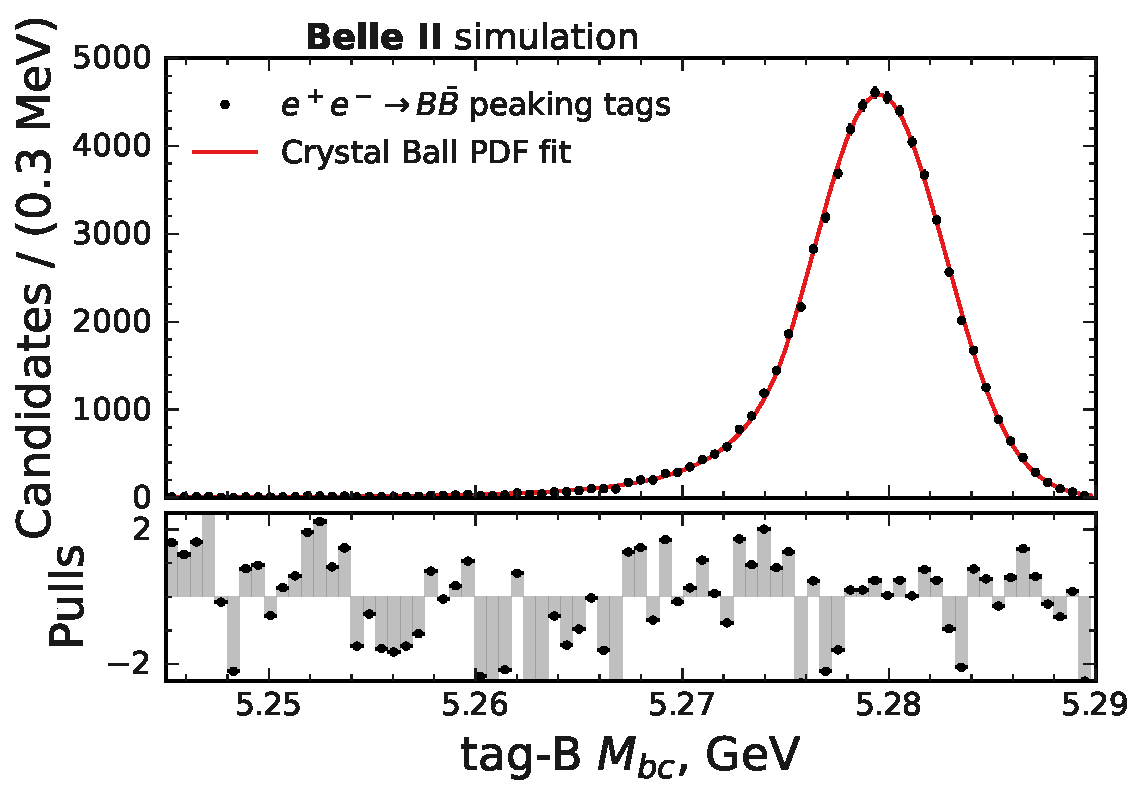
\includegraphics[width=0.3\textwidth]{figures/fitting/mbc_good_tags_fit.pdf}
    }
    \subcaptionbox{\label{fig:combinatorial_tags_fit}}{
        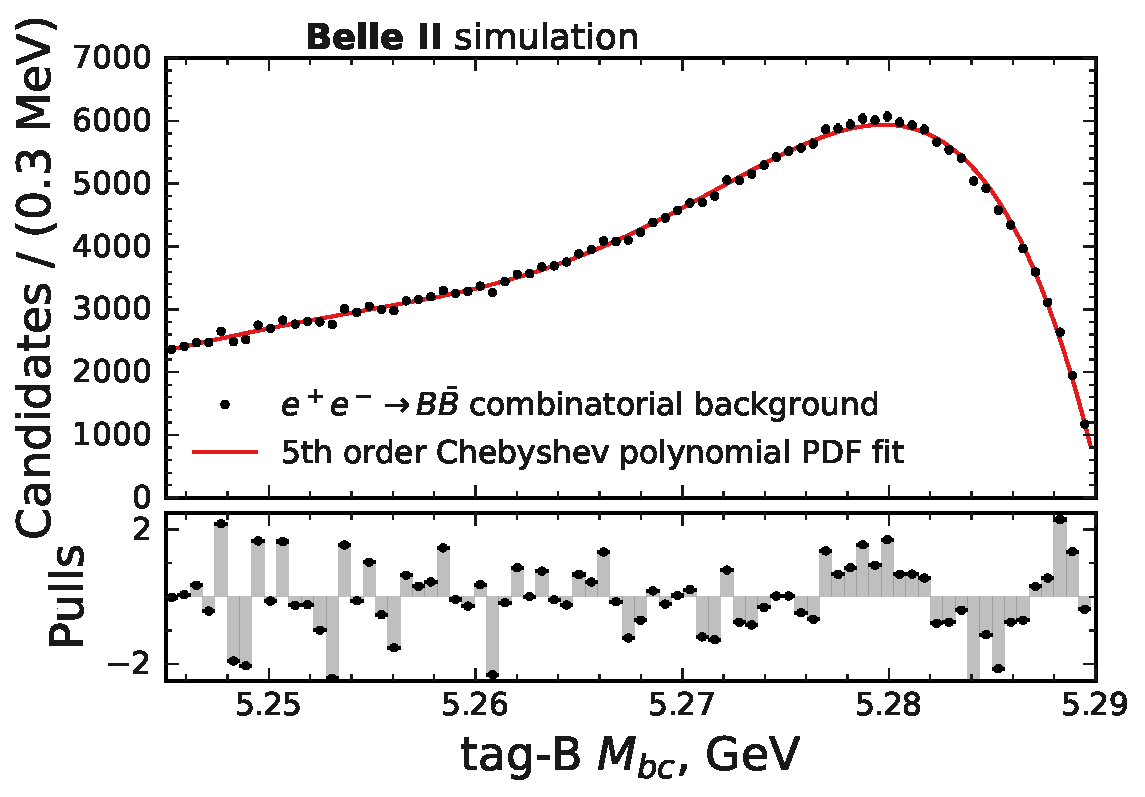
\includegraphics[width=0.3\textwidth]{figures/fitting/mbc_combinatorial_tags_fit.pdf}

    }
    \subcaptionbox{\label{fig:argus_tags_fit}}{
        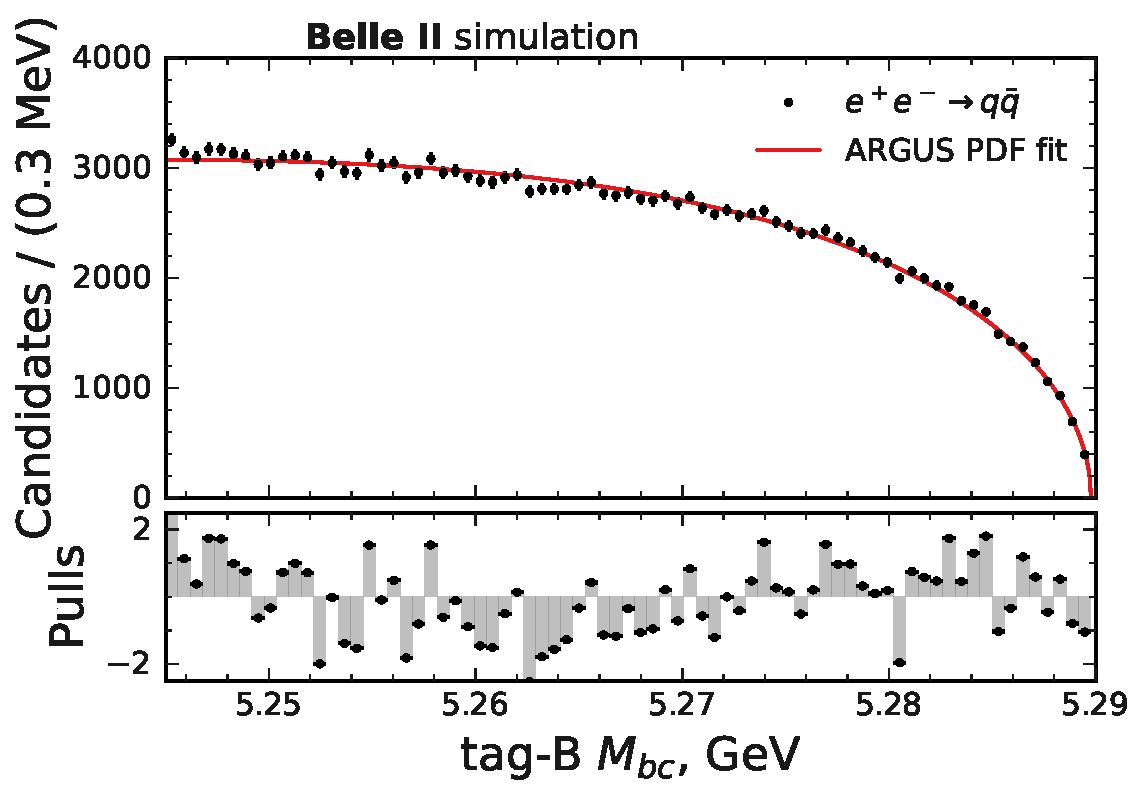
\includegraphics[width=0.3\textwidth]{figures/fitting/mbc_continuum_tags_fit.pdf}
    }
    \caption{\label{fig:tag_component_fits} Separate components that are present in generic \MC after selections that suppress background (\Cref{tab:cutflow}).
    The individual components are defined in \Cref{sec:fitting_components} text.
    Each distribution contains an unbinned illustrative fit to the data points, and the subpanels show the pull (\Cref{eq:pull_distribution}) in each case.
    The fitting function for peaking tag \B mesons (\Cref{fig:good_tags_fit}) is chosen as the Crystal Ball function;
    for combinatorial tag \B mesons (\Cref{fig:combinatorial_tags_fit}) it is chosen as the 5th order Chebyshev;
    for continuum \epem\ra\qqbar events (\Cref{fig:argus_tags_fit}) it is chosen as the ARGUS function.
    }
\end{figure}

The fitting model is prepared to describe the three components and, particularly, to extract the number of tag-$B$ candidates that corresponds to the `peaking' component.
The strategy to describe each component is as follows:
\begin{itemize}
    \item Peaking \Mbc distributions are often fitted using a Crystal Ball function.
    It is defined in \Cref{sec:crystal_Ball}, but can be understood as Gaussia distribution with a polynomial tail.
    \Cref{fig:good_tags_fit} illustrates the suitability to describe the peaking \Mbc distribution.
    \item Continuum \Mbc distributions are conventionally described by the ARGUS function, which is named after the ARGUS collaboration and designed specifically for this purpose;
    This function, utilised to describe \epem\ra\qqbar simulated backgrounds in this analysis is seen in \Cref{fig:argus_tags_fit}.
    \item The particular shape of the combinatorial \BB background is generally dependant on the signal mode and do not have a conventional method of description.
    In this analysis, the usage of \FEI and the fact that background events are conservatively suppressed to avoid signal-side biases leads to an wide but slightly peaking shape.
    Several options were assessed in this ana;lysis, but it was found that it is suitably described by a Chebyshev polynomial, which can be adapted to a necessary functional shape.
    This is illustrated in \Cref{fig:combinatorial_tags_fit}, where a 5th order polynomial describes the combinatorial \BB background distribution.
\end{itemize}
In \Cref{fig:tag_component_fits} the subpanels shown the pull distribution, which is defined as:
\begin{equation}\label{eq:pull_distribution}
    \mathrm{pull}(x) = \frac{x-\mu}{\sigma}. 
\end{equation}
Throughout this thesis it is used to evaluate the quality of the fit, as repeated measurements of a random variable $x$ should fluctuate around a mean value $\mu$ with a possonian width $\sigma$.
Therefore any dependancies or strucutes observed in the pull distribution would be indicators of poor fit quality. 

\subsection{Photon energy intervals for the fit}\label{sec:binning}

It is clear from \Cref{fig:spectrum_after_optimisation} that signal-to-background ratio changes across all \EB range.
In fact, even continuum-to-\BB event fractions are not constant.
This is a result of the fact that photons related to \epem\ra\qqbar backgrounds are more likely to extend to high-\EB values, because they do not originate from a \B meson which is always produced with $\sqrt{s}/2$ at Belle II.
The goal of the fit, as discussed in the introduction of this Section, is to remove combinatorial \BB and continuum events from further analysis.
While an overall \Mbc fit could be performed, such an approach necessarily loses event-level information, such as the energy of each individual photon, and only provides the event-counts in the fitted \EB region.
Furthermore, the fact that the background composition is expected to vary with \EB, such an overall-fit may generally be suboptimal.

Instead, in this analysis the photon spectrum is divided into multiple \EB intervals, and the \Mbc distributions belonging to each interval are fitted using the functions described in \Cref{sec:fitting_components}.
This approach will then reduce the existing dataset to multiple \EB intervals with known good tag-\B counts, completely removing continuum and combinatorial \BB events from the dataset.
Such an approach means that the final photon-energy spectrum will be provided in the binning used for fitting.
It is therefore important to optimise the chosen intervals for the fit with respect to expected \BtoXsgamma in each interval, despite the fact that the primary goal of the fit is not signal extraction.
For the rest of the thesis, \EB intervals will be referred to as \EB bins.

Three scenarios are tested for $\EB\in(1.4,2.8)~\gev$: 50~\mev, 100~\mev and 200~\mev wide bins.
The test is performed by evaluating the statistical significance, with a definition equivalent to \Cref{eq:soversqrtsplusb}, on a dataset scaled to 200~\invfb.
In this case, the background is considered what is anticipated after the \Mbc fit: only correctly-tagged \BB events (no combinatorial or continuum background).
The result of the study of statistical significance for the hybrid signal model (\Cref{sec:signal_model}) is shown in \Cref{fig:binning_significance}.

\begin{figure}[htbp!]
    \centering
    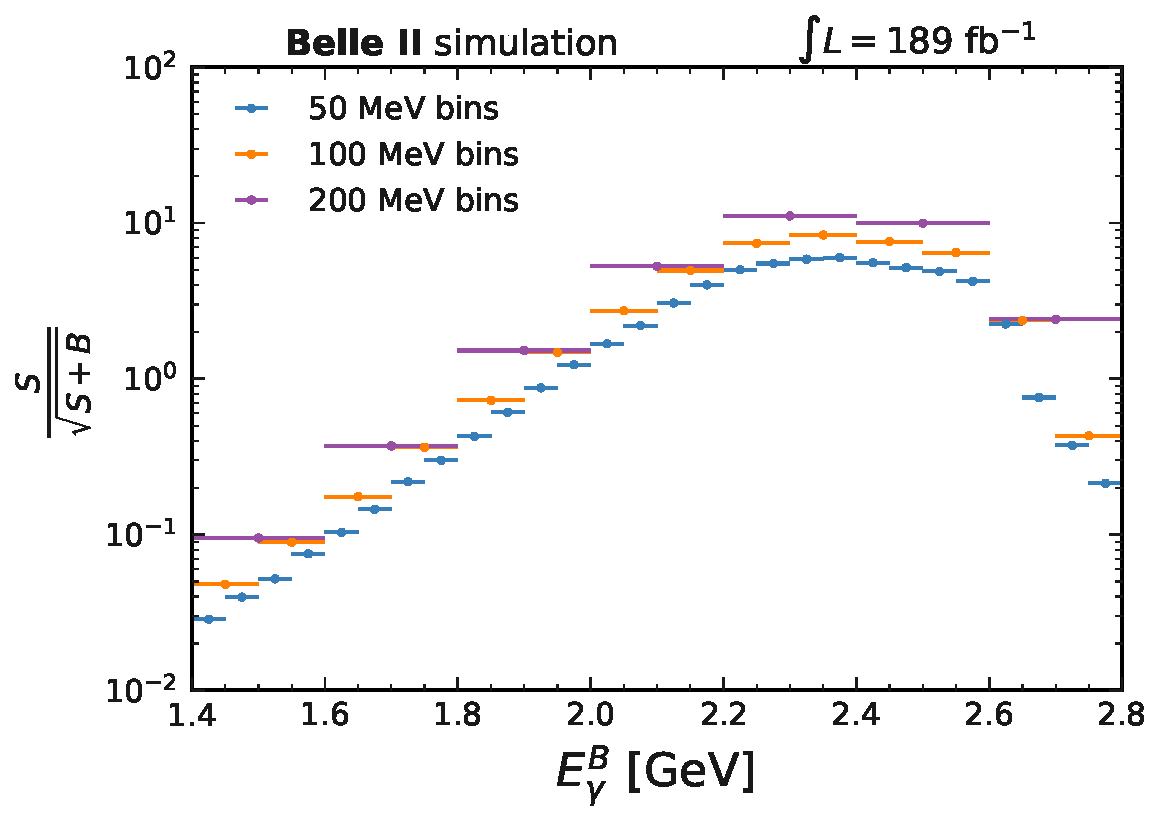
\includegraphics[width=0.5\textwidth]{figures/fitting/binning_significance.pdf}
    \caption{\label{fig:binning_significance}The results of statistical significance, based on \Cref{eq:soversqrtsplusb}.
    Here the $S$ is takes as number of \BtoXsgamma events after fitting and $B$ is taken as non-\BtoXsgamma events expected after fitting in each \EB interval.
    Three scenarios are tested: 50~\mev, 100~\mev and 200~\mev wide bins.
    The final binning chosen is a hybrid scenario described in \Cref{sec:binning} text.
    The hybrid model described in \Cref{sec:signal_model} is used for this study.
    }    
\end{figure}

In general, the highest statistical significance is observed with the widest bins, but this method, by definition, contains the least amount of information about the spectrum.
Irrespective of the bin-width,  $\EB\in(1.4,1.8)$ and $\EB>2.6$ show a statistical significance lower than unity, therefore the selected binning should attempt to maximise it.
In the case of $\EB\in(1.8,2.0)$ bin, it is observed that a similar statistical significance can be achieved a with $\EB\in(1.9,2.0)$ bin.
This motivates to extend it, such that an \EB threshold of 1.8~\gev could be achieved, as opposed to the 1.9~\gev threshold in Ref.\cite{BaBar:2007yhb}.
Later studies performed in XXX showed that the resolution of \EB is expected to be roughly 30~\mev.
The similarity between resolution and \EB can lead to complications in the unfolding procedure.
Due to the fact that bin-by-bin unfolding is employed in this analysis, the 50~\mev bins were not considered.

These considerations led to choosing the following eleven \EB bins for the analysis:
\begin{itemize}
    \item Three 200~\mev bins for $\EB\in(1.4,2.0)$;
    \item Seven 100~\mev bins for $\EB\in(2.0,2.7)$;
    \item A single, inclusive overflow bin $\EB>2.7$.
\end{itemize}
This choice provides a compromise between statistical significance, \EB spectrum resolution and complications in unfolding.
The expected continuum, combinatorial, correctly-tagged non-\BtoXsgamma $BB$ and correctly-tagged \BtoXsgamma event count expectations for the chosen binning are provided in \Cref{tab:expected_events}.
Note that the table entry containing combinatorial \BB includes also \BtoXsgamma events, even if it is considered background in the \Mbc fits in XX.
On the other hand peaking-\BB background, which is not rejected by the \Mbc fit and will be treated in XXX, is separated from \BtoXsgamma.
The table also highlights the importance of a correct binning, as it is obvious that several bins are able to achieve a comparable statistical significance to the one that could be achieved if just a single bin was used.

\begin{table}[htbp!]
    \caption{\label{tab:expected_events}Expected number of events as a fraction of the dataset after selections in \Cref{tab:cutflow}, for the binning chosen in \Cref{sec:binning}.
    The table also shows corresponding statistical significance for a 200~\invfb sized dataset.
    }
    \resizebox{1\textwidth}{!}{
\begin{tabular}{|l|lllll|}
\hline
\EB bins [\gev] & Continuum frac. & Combinatorial \BB (incl. \BtoXsgamma) & Peaking \BB frac (excl. \BtoXsgamma) & Peaking \BtoXsgamma & $\frac{S}{\sqrt{S+B}}$ at 189~\invfb \\
\hline
$1.4-1.6$ &    0.22 &       0.20 &   0.047 &  0.00010 & 0.1 \\
$1.6-1.8$ &    0.14 &      0.094 &   0.028 &  0.00031 & 0.38 \\
$1.8-2.0$ &    0.088 &      0.046 &   0.016 &   0.00097 &  1.56 \\
$2.0-2.1$ &   0.028 &      0.013 &  0.0048 &   0.0010 &    2.80 \\
$2.1-2.2$ &    0.020 &     0.0079 &  0.0026 &   0.0016 &  5.05 \\
$2.2-2.3$ &   0.013 &     0.0048 &   0.00093 &   0.0019 &  7.5 \\
$2.3-2.4$ &  0.0075 &     0.0033 &  0.00031 &    0.0019 &   8.4 \\
$2.4-2.5$ &  0.0042 &     0.0019 &  0.00024 &   0.0015 &   7.6 \\
$2.5-2.6$ &  0.0019 &    0.00062 &  0.00013 &    0.0011 &  6.5 \\
$2.6-2.7$ & 0.00059 &    0.000098 & 0.000016 &  0.00014 &  2.38 \\
$2.7-5.0$ & 0.00021 &     0.000011 &   $<0.000001$ &  0.000005 & 0.46 \\
\hline
All        &    0.52 &       0.37 &    0.10 &    0.011     &   6.61 \\
\hline
\end{tabular}
}
\end{table}

Because of the low expected statistical significance, the $\EB\in(1.4,1.8)$ and $\EB>2.7~\gev$ are chosen as validation regions.
They will later be referred to as \textit{sidebands}.
Consequentially, the signal region of the study is defined as $\EB\in(1.8,2.7)$.

\todo[inline]{If there is time transform this to 189 invfb, otherwise include why I am not doing that, eg it was the size the analsys was thought to be applied on etc etc.}

\subsection{Fit model building}\label{sec:fitting_setup}

The functions introduced in \Cref{sec:fitting_functions} are now considered in terms of the defined binning in \Cref{sec:binning}.
Using them an overall fit model build.
However, the implementation of an $N$-th order Chebyshev polynomial, a Crystal Ball function and an ARGUS function for every \EB bin is unreasonable:
this would result in $N+6$ model parameters and 3 normalisation parameters for each bin.
Therefore, first, a fit model version, where some of the parameters can be pre-determined or shared amongst the bins is prpared.

Firstly, all the functions are fitted once, separately, on the subsets of the simulated that they aim to describe.
This is done in order to estimate the starting parameters that will be used on the fit of the total (combined) dataset.
The first fit is discussed separately for each component.

\todo[inline]{fill XXX in each to show a table of final parameters for each PDF}

\subsubsection{Crystal Ball function}\label{sec:crystal_ball_prefit}

The Crystal Ball function, describes the distribution of `good' tag-\B mesons in \Mbc.
In principle, the tag-\B meson is an independent object from the signal-\B meson decays -- which means that no strong \EB correlation is expected.
This hypothesis is tested in \Cref{fig:crystal_ball_par_test}.
It can be seen that strong correlations between \EB and parameters $\mu$ and $\sigma$ are absent.
This test is not performed on parameters $\alpha$ and $n$, as they tend to be less-stable than $\mu$ and $sigma$ and depend more on fluctuations of the dataset.
It is therefore concluded, that a single \Mbc shape for \EB bins will be used, with the parameters pre-determined in a total fit (\Cref{fig:good_tags_fit}).
The values and uncertainties from the fitter, are shown in XXX.

\begin{figure}[htbp!]
    \subcaptionbox{\label{fig:crystal_ball_mus}}{
        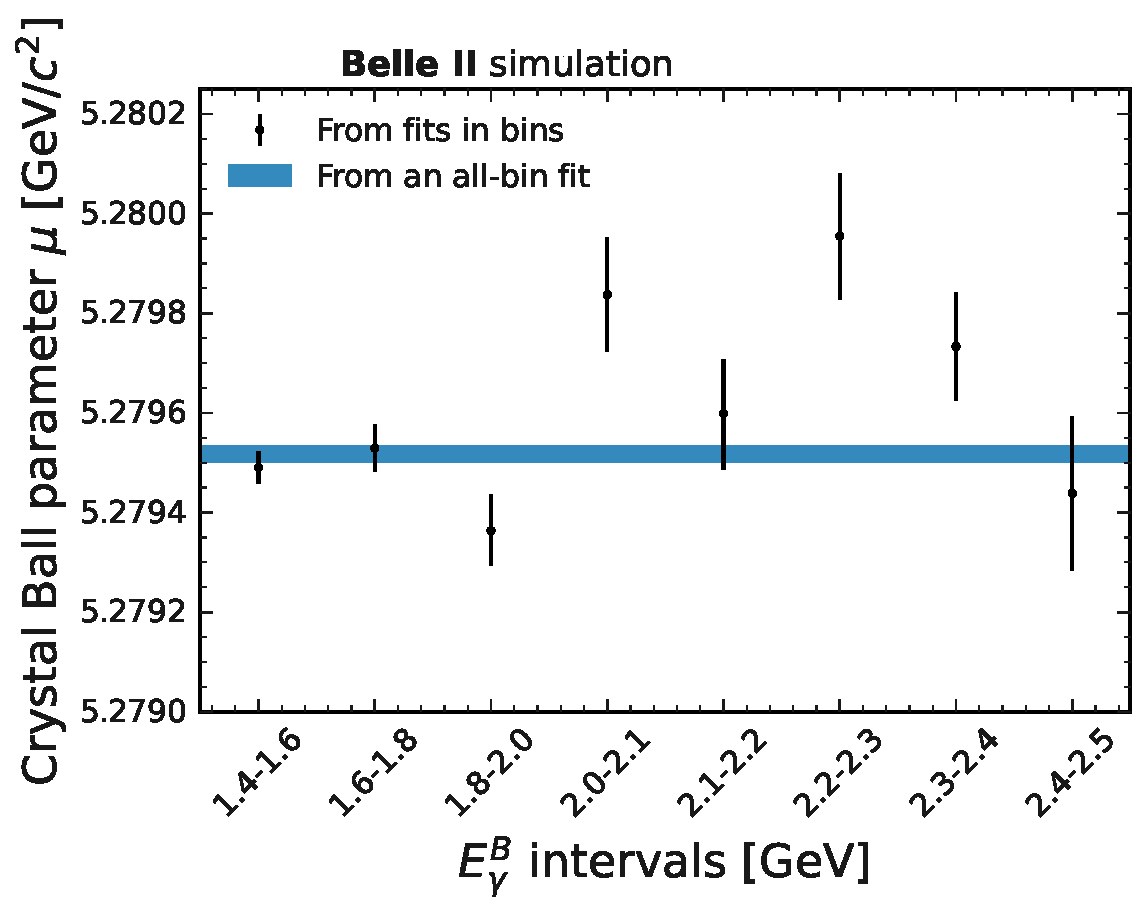
\includegraphics[width=0.4\textwidth]{figures/fitting/Crystal_Ball_PDF_test_mu.pdf}
    }
    \subcaptionbox{\label{fig:crystal_ball_sigmas}}{
        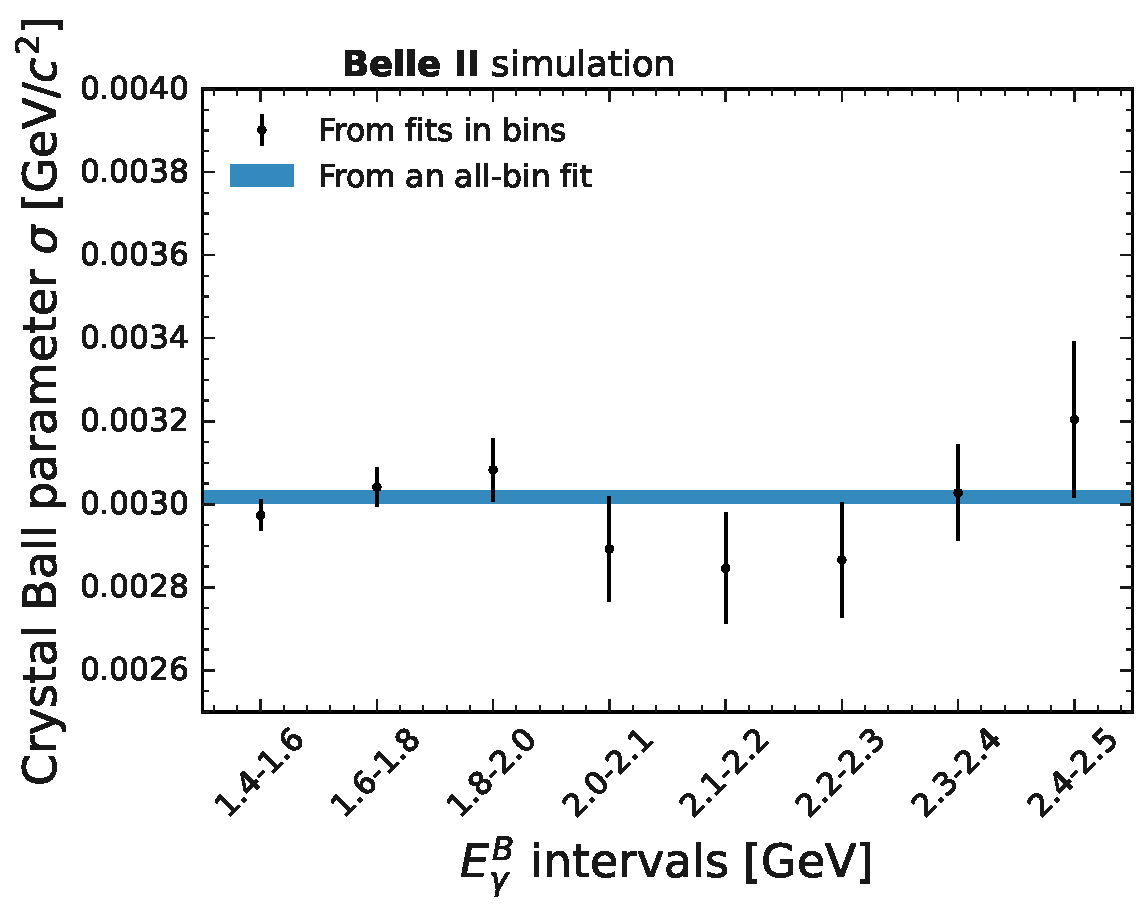
\includegraphics[width=0.4\textwidth]{figures/fitting/Crystal_Ball_PDF_test_sigma.pdf}
    }
    \caption{\label{fig:crystal_ball_par_test}The parameters from \Mbc fits of `good' tag-\B mesons in generic-\BB simulation, using a Crystal Ball function.
    The datapoints showcase the estimated parameters $\mu$ (\Cref{fig:crystal_ball_mus}) and $\sigma$ (\Cref{fig:crystal_ball_sigmas}) for different
    \EB intervals.
    This can be compared with the overall shape (blue band), that is determined if the entire $\EB\in(1.4,2.8)$ region is fitted.
    The parameters of the blue band correspond to the fit in \Cref{fig:good_tags_fit}.
    No strong dependance on \EB is observed.
    }
\end{figure}

\subsubsection{Chebyshev polynomial function}\label{sec:chebyshev_prefit}

The Chebyshev \PDF takes $N$ parameters as coefficients scaling each order of the polynomial that goes into the fitting function (\Cref{eq:chebyshev_pdf}).
The $N$ is therefore referred to as the \textit{order} of the Chebyshev \PDF.
3-rd, 4-th and 5-th order Chebyshev polynomials are tested for suitability to describe the combinatorial \BB background distribution.
The 5-th order result is already introduced in \Cref{fig:combinatorial_tags_fit}.
The results of the best fit for lower-order polynomials is presented in \Cref{fig:lower_order_chebyshev}.
From the pull distributions in the subpanels and the general inspection of the fit, it is clear that using a polynomial of order lower than 5 is insufficient for an adequate description of combinatorial \BB events.

\begin{figure}[htbp!]
    \subcaptionbox{\label{fig:3rd_order_chebyshev}}{
        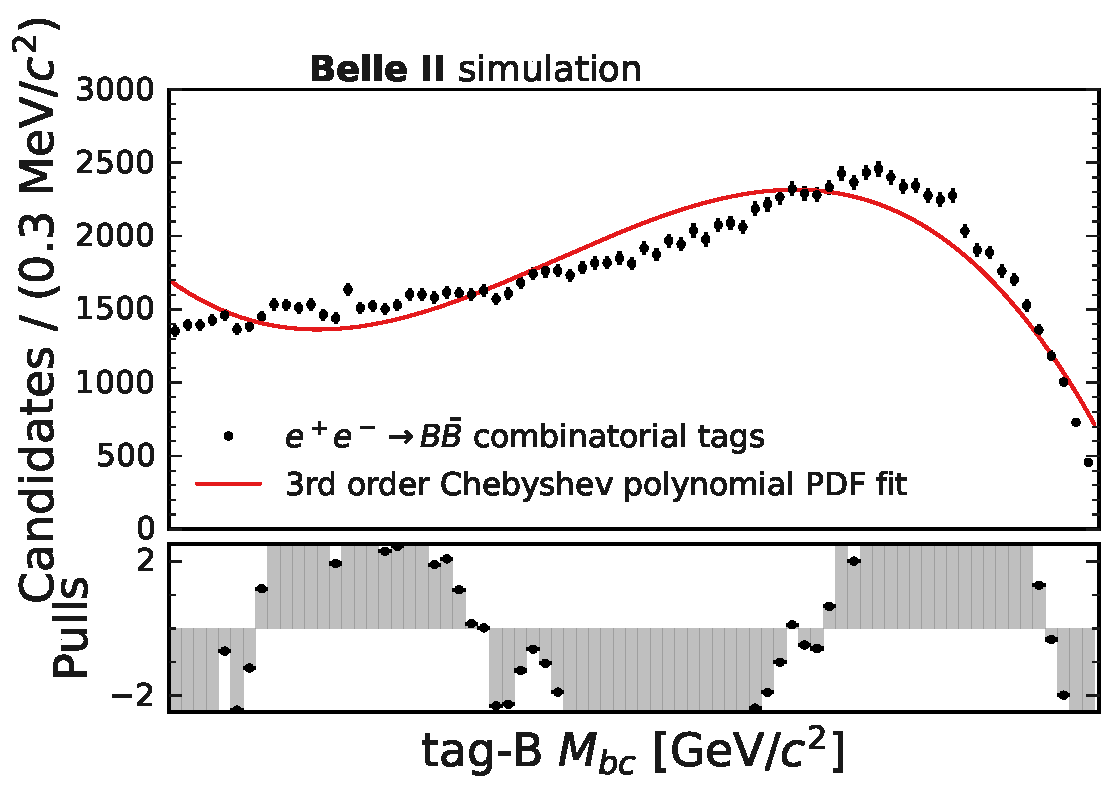
\includegraphics[width=0.4\textwidth]{figures/fitting/3rd_order_chebyshev_polynomial.pdf}
    }
    \subcaptionbox{\label{fig:4th_order_chebyshev}}{
        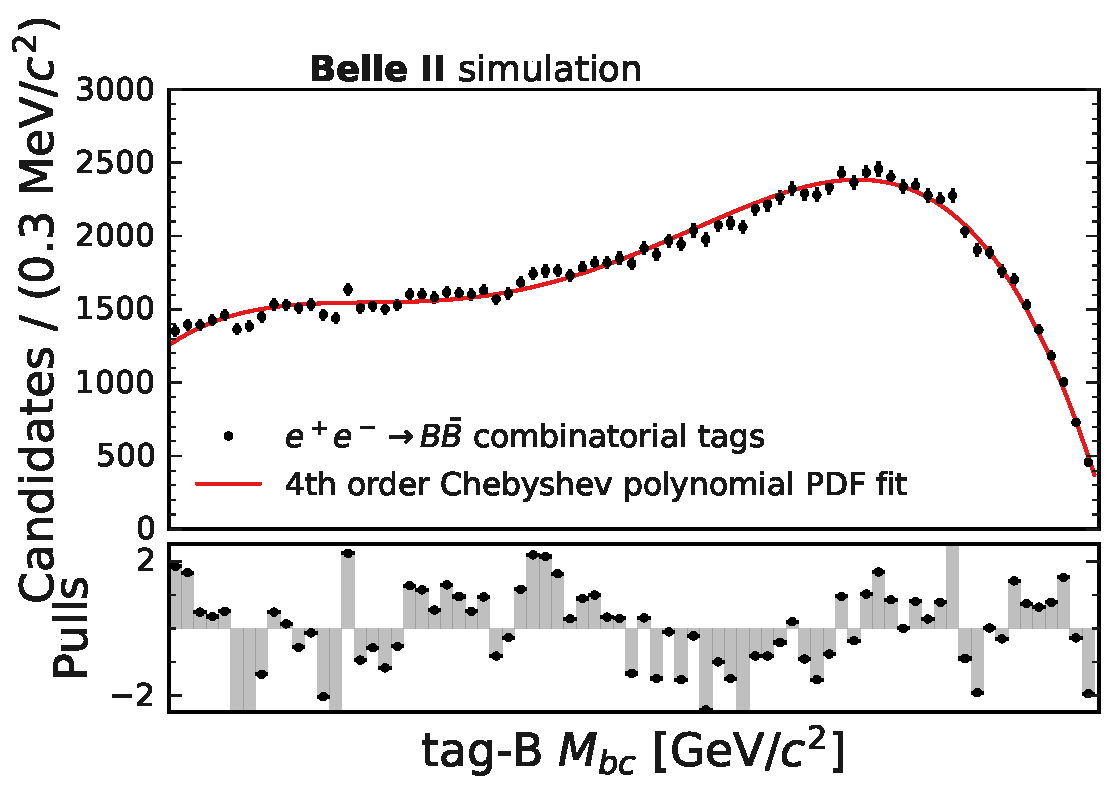
\includegraphics[width=0.4\textwidth]{figures/fitting/4th_order_chebyshev_polynomial.pdf}
    }
    \caption{\label{fig:lower_order_chebyshev}The \Mbc fits of combinatorial \BB events when a Chebyshev \PDF of order 3 (\Cref{fig:3rd_order_chebyshev}) or 4 (\Cref{fig:4th_order_chebyshev}) is used.
    These figures can be compared to \Cref{fig:combinatorial_tags_fit}.
    It is clear that lower order Chebyshev polynomials are unable to accurately describe the combinatorial-\BB data.
    }
\end{figure}


The coefficients $c_{1-5}$ of the Chebyshev polynomial cannot be easily connected to physics observables,
and therefore it is hard to evaluate their dependance on \EB.
As such, 3 different PDFs are chosen: $\EB\in(1.4,1.6)$, $\EB\in(1.6,1.8)$, $\EB>1.8$ \gev.
The reason why the last interval is not subdivided further is because of the dataset size -- each interval was optimised to have a roughly equal number of events, to minimize statistical fluctuations related to the shape determination.
The Chebyshev \PDF parameters for each interval are determined in an \Mbc fit on the appropriate region and fixed for the fit of the total dataset later.

\subsubsection{ARGUS function}\label{sec:argus_prefit}
